\documentclass[a4paper, 12pt, final, garamond]{book}
\usepackage{cours-preambule}

\makeatletter
\renewcommand{\@chapapp}{Devoir surveill\'e -- num\'ero}
\makeatother

\begin{document}
\setcounter{chapter}{4}

\chapter{Commentaires sur le DS n\degree05}

\section{Commentaires généraux}

Des techniques d'adimensionnement random. J'avais insisté sur le fait qu'on vous
le demande si nécessaire~: ne vous compliquez pas la vie pour rien~!

% \begin{figure}[htbp!]
% 	\centering
% 	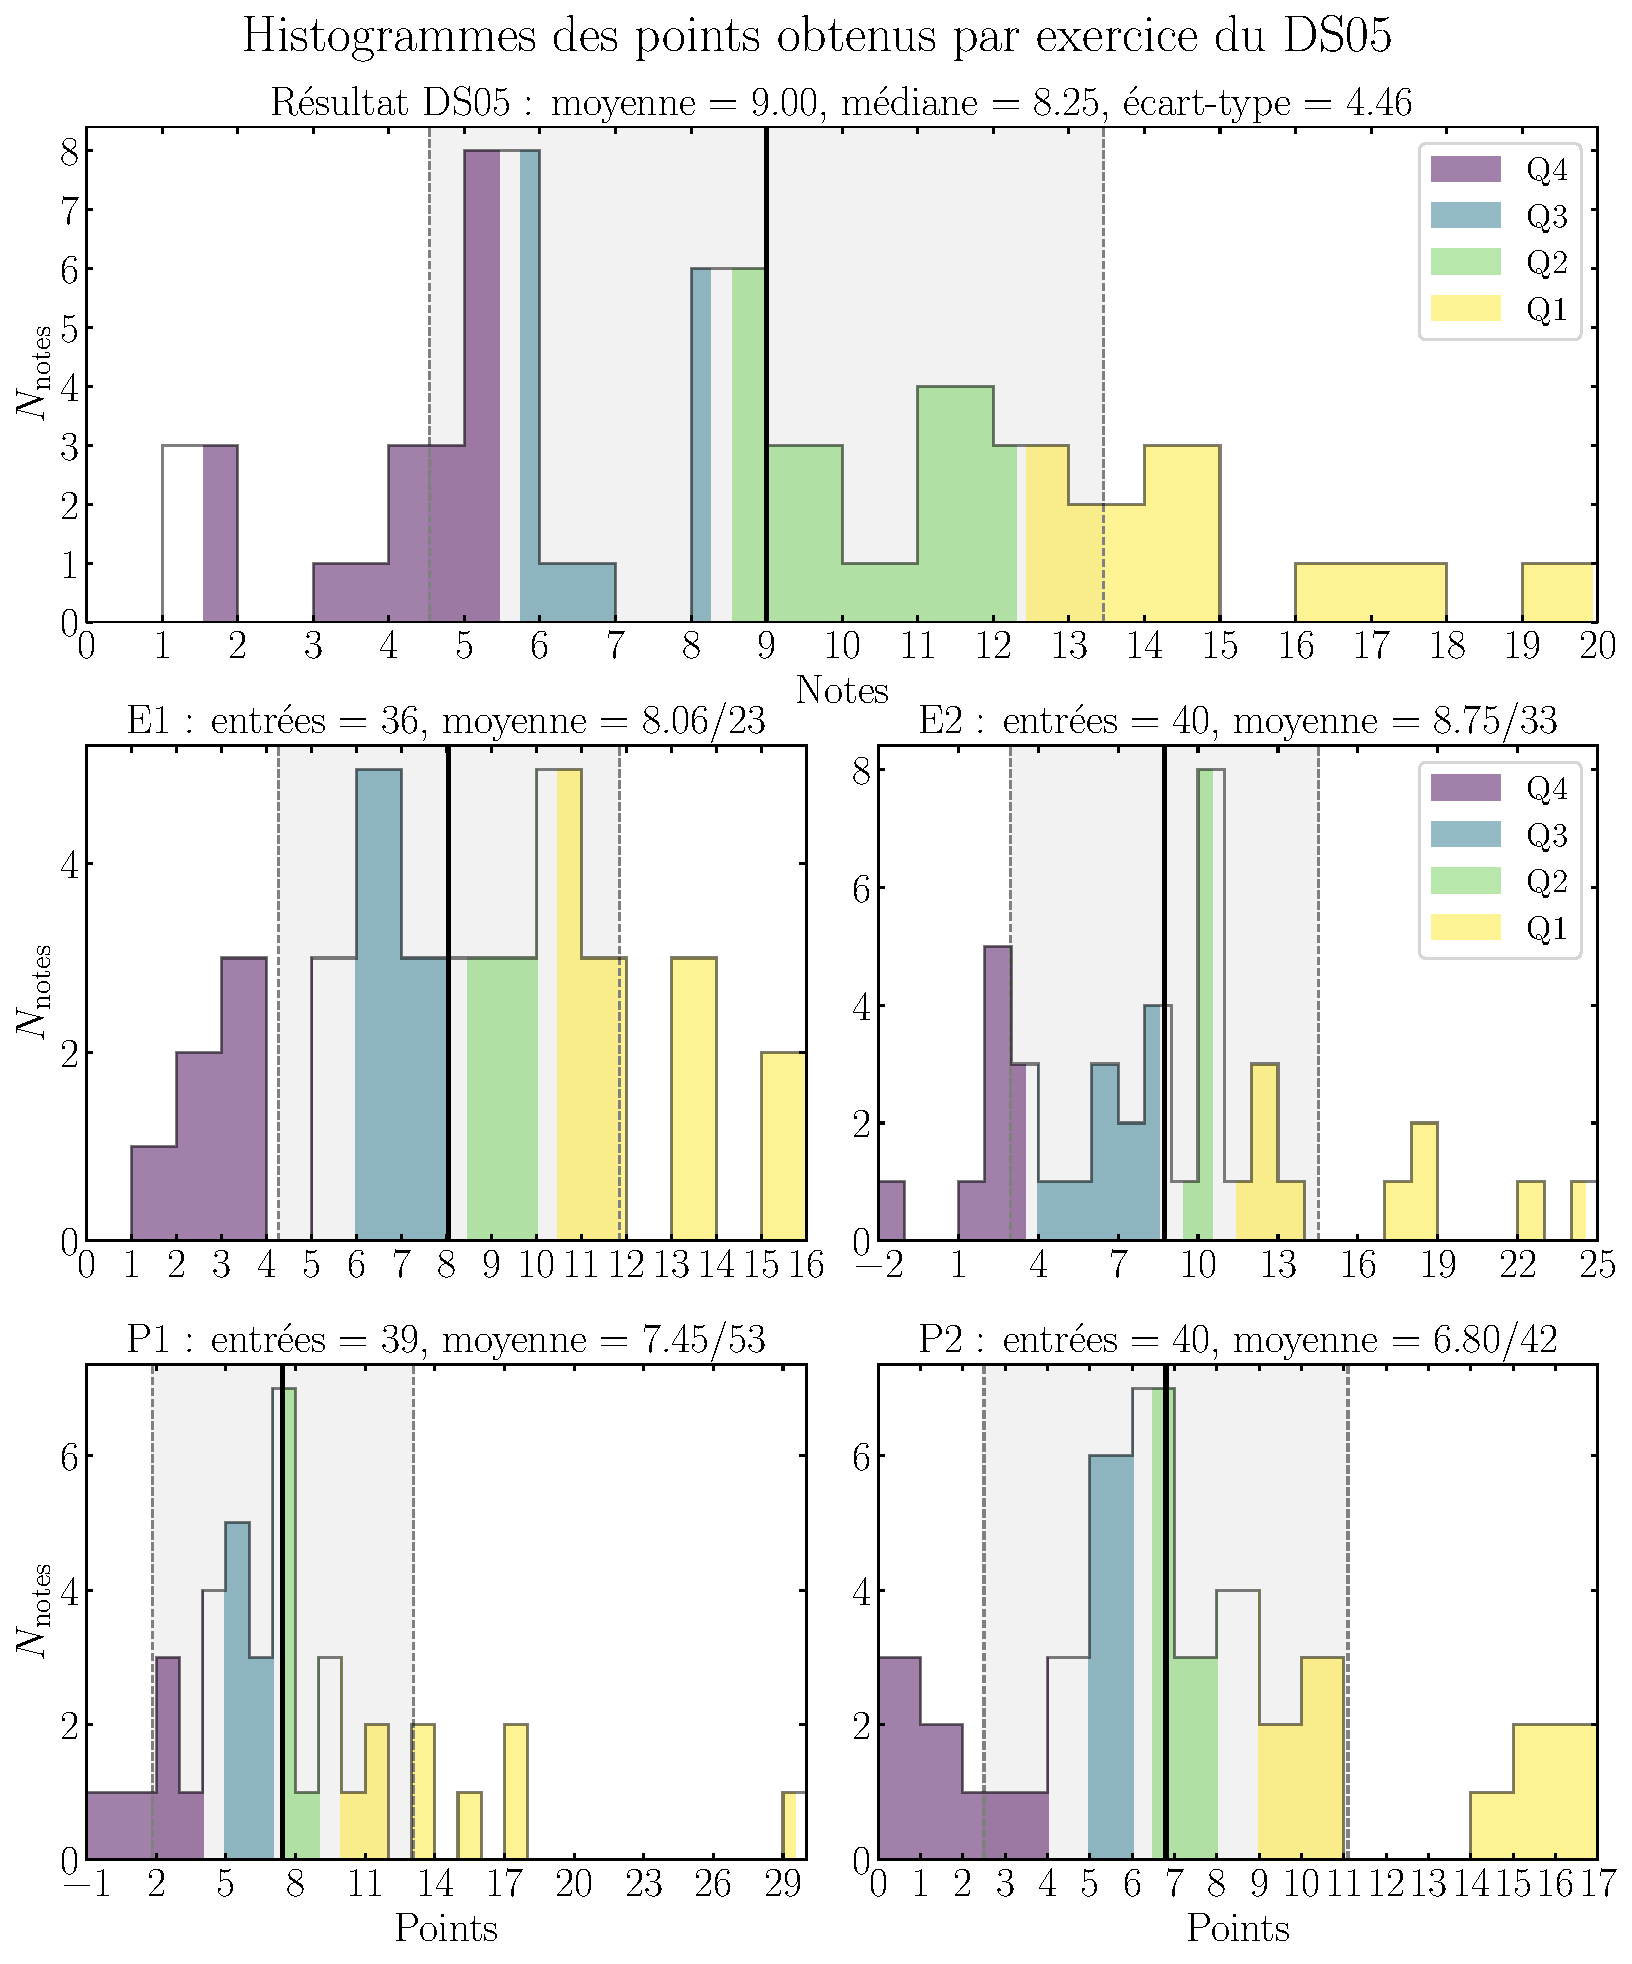
\includegraphics[width=\linewidth]{DS05_hist_all}
% 	\caption{Graphique des résultats}
% \end{figure}

\setcounter{section}{0}
\exercice[22]{Ondes gravitationnelles}
\begin{enumerate}
	\nitem{6} % Q1
	Trop incomplet. Même nature et même fréquence avant toute chose, cohérence
	ensuite.
	\nitem{2} % Q2
	Correct.
	\nitem{5} % Q3
	Il fallait partir du retard temporel. \textbf{N'ajoutez pas des phases à
		l'origine} quand on vous a explicitement donné la forme du signal à l'origine.
	\nitem{1} % Q4
	RAS.
	\nitem{1} % Q5
	RAS.
	\nitem{3} % Q6
	Correct.
	\nitem{3} % Q7
	Ne confondez pas le terme de phase à l'origine dans le signal sinusoïdal avec
	le déphasage dans l'amplitude du signal !
	\nitem{3} % Q8
	RAS.
\end{enumerate}

\exercice[33]{Chute d'une bille}
\begin{enumerate}
	\nitem{2} % Q1
	Poussée d'\textsc{Archimède} non connue. Aïe. Vous oubliez l'accélération de
	la pesanteur $\gf$~!
	\nitem{4} % Q2
	Réponses variées.
	\nitem{7} % Q3
	Globalement correct, mais vos schémas doivent faire apparaître les forces sur
	le système et le BDF doit être exprimé dans le repère choisi~! \textbf{Vous
		oubliez trop le repérage}.
	\nitem{3} % Q4
	Certain-es ont considéré que la bille avait changé de masse, et ont utilisé la
	masse volumique $\rho$ en facteur de $\af$ \textbf{et} en facteur de $\gf$… ça
	n'a aucun sens.
	\nitem{6} % Q5
	En fonction des données du problème, donc pas de $m$ qui n'est pas donné, mais
	du $4/3\,\pi R^{3}$~!
	\nitem{5} % Q6
	\nitem{1} % Q7
	\nitem{3} % Q8
	\nitem{2} % Q9
\end{enumerate}

\setcounter{section}{0}
\prblm[53]{Microphone pour guitare}
\begin{enumerate}
	\nitem{6} % Q1
	Infiniment déçue des «~intensité nulle donc tension nulle~» pour un
	interrupteur ouvert… c'est accablant. Travaillez sincèrement les premières
	questions de régime permanent.
	\nitem{4} % Q2
	Il faut savoir faire le PdT dans le bon sens~!!
	\nitem{7} % Q3
	Soyez malin-es : $H_0$ ne dépend pas de $\w$. Il faut savoir identifier des
	expressions variables et constantes dans une équation. Ne vous précipitez pas
	pour dire $\w_0 = 1/\sqrt{LC_0}$ si ça n'est pas une évidence~: on identifie
	\textbf{après}~!
	\nitem{7} % Q4
	Vous n'avez pas retenu ce qu'est la résonance. Fâcheux.
	\nitem{10} % Q5
	Souvent faux parce que c'était un passe-bas.
	\nitem{2} % Q6
	RAS.
	\nitem{2} % Q7
	RAS.
	\nitem{1} % Q8
	Il faut connaître ses définitions et vocabulaire…
	\nitem{5} % Q9
	RAS.
	\nitem{6} % Q10
	RAS.
	\nitem{3} % Q11
	RAS.
\end{enumerate}

\prblm[42]{Le bleu du ciel}
\begin{enumerate}
	\nitem{4} % Q1
	Dimensions $\neq $ unités !
	\nitem{2} % Q2
	Bien.
	\nitem{4} % Q3
	TB.
	\nitem{2} % Q4
	\nitem{9} % Q5
	\nitem{2} % Q6
	\nitem{4} % Q7
	\nitem{3} % Q8
	\nitem{1} % Q9
	\nitem{2} % Q10
	\nitem{1} % Q11
	\nitem{2} % Q12
	\nitem{2} % Q13
	\nitem{2} % Q14
	\nitem{2} % Q15
\end{enumerate}

\end{document}
